\documentclass[11pt,notes=hide,aspectratio=169,mathserif]{beamer}

% ================= PREAMBLE (matches your style) =================
\usepackage{graphics}
\usepackage{graphicx}
\usepackage{url}
%\usepackage{natbib}
\usepackage{bibentry}
\usepackage{verbatim}
\usepackage{booktabs}
\usepackage{etoolbox}
\usepackage{datetime}
\usepackage{bm}
\usepackage{subcaption}
\usepackage{amsfonts}
\usepackage{amsmath}
\usepackage{amsthm}

\def\newblock{}
\linespread{1.2}

\title[class]{ECON 340: Economics of the Family \\ TA Session 7}
\author[Vaidehi's class]{Vaidehi Parameswaran (Northwestern Economics)}
\date{\monthname[\the\month] \the\year}

\usetheme{metropolis}
\definecolor{mycolor}{RGB}{48,7,144}
\setbeamercolor{frametitle}{bg=mycolor, fg=white}
\setbeamercolor{title separator}{fg=mycolor}
\setbeamercolor{progress bar}{fg=mycolor}
\beamertemplatenavigationsymbolsempty
\setbeamertemplate{footline}[frame number]{}
\setbeamertemplate{itemize item}{\small\raisebox{1pt}{\textcolor{mycolor}{$\blacktriangleright$}}}
\setbeamertemplate{itemize subitem}{\footnotesize\raisebox{1pt}{\textcolor{mycolor}{$\triangleright$}}}
\setbeamertemplate{itemize subsubitem}{\tiny\raisebox{1pt}{\textcolor{mycolor}{$\triangleright$}}}

\usepackage{hyperref}
\hypersetup{
  colorlinks=true,
  linkcolor=mycolor,
  urlcolor=mycolor,
  citecolor=mycolor
}

\usepackage{appendixnumberbeamer}
\setbeamertemplate{section in toc}{%
  \leavevmode\llap{\textcolor{mycolor}{$\blacktriangleright$}\hspace{0.6ex}}%
  \inserttocsection\par}
\setbeamertemplate{subsection in toc}{%
  \leavevmode\llap{\textcolor{mycolor}{$\triangleright$}\hspace{1.1ex}}%
  \inserttocsubsection\par}

\AtBeginSection[]{
  \begin{frame}{Today}
    \tableofcontents[currentsection]
  \end{frame}
}

\begin{document}

% ---------------------------------------------------------------
\begin{frame}[plain]
\titlepage
\end{frame}
% ---------------------------------------------------------------


\section{Parental Leave Benefits, Household Labor Supply, and Children’s Long-run Outcomes}

% ---------------------------------------------------------------
\begin{frame}{Today's Paper}
\small
\textbf{Ginja, Jans \& Karimi (2018).} \emph{Parental Leave Benefits, Household Labor Supply, and Children’s Long-run Outcomes} (Sweden).\\[0.6em]
\textbf{Question:} How do \emph{benefit levels} in parental leave (holding duration \& job protection fixed) affect\\
\hspace{1.2em}(i) mothers’ and partners’ labor supply and household income, and\\
\hspace{1.2em}(ii) older vs.\ younger siblings’ health \& education?\\[0.4em]
\textbf{Design:} RD at Swedish \textbf{Speed Premium (SP)} spacing cutoffs (24 and 30 months) for consecutive births.
\end{frame}
% ---------------------------------------------------------------


% ---------------------------------------------------------------
\begin{frame}{Swedish Parental Leave \& the Speed Premium}
\small
\begin{itemize}
  \item 1970s–80s Sweden: paid, job-protected parental leave (PL); wage-replaced benefits (about 90\% of prior salary, capped).
  \item \textbf{Work requirement} (qualifying earnings) usually needed to set the benefit level for the next child.
  \item \textbf{Speed Premium (SP):} if births are spaced within a threshold, the mother keeps the \emph{previous} wage-based benefit \emph{without re-qualifying}.
  \begin{itemize}
    \item Threshold set to \textbf{24 months} (1980–85), then \textbf{30 months} (1986–).
    \item Eligibility determined using \emph{expected due date}; revealed during pregnancy.
  \end{itemize}
  \item Thus implied that mothers did not have to return to work between births and re-qualify for (higher) PL benefits,
\end{itemize}
\end{frame}
% ---------------------------------------------------------------


% ---------------------------------------------------------------
\begin{frame}{So what does the SP do?}
\small
\pause 
\begin{itemize}
  \item Intuition: SP lowers the opportunity cost of home time \emph{before and after} the subsequent birth.
  \item Incentives for mothers to space births in short intervals
  \item So mong mothers with at
  least one child, giving birth to a subsequent child outside of the eligibility spacing interval implies a lower benefit level for leave taken with the new child
\end{itemize}
\end{frame}
% ---------------------------------------------------------------

% ---------------------------------------------------------------
\begin{frame}{Data \& Outcomes}
\small
\begin{itemize}
  \item Linked Swedish registers (parents \& children): labor earnings, disposable income, births, health (inpatient), grade 9 GPA, high school eligibility, college by age 24.
  \item \textbf{Sample:} families with \(\ge\)2 children; main window \(\pm24\) weeks around the cutoff; second births 1980–89.
  \item \textbf{Parent outcomes:} mothers’/fathers’ labor earnings (pre- and post-birth windows), maternal participation, household disposable income.
  \item \textbf{Child outcomes:} birth outcomes (younger child), hospitalizations at ages 10/14, education (GPA, high school eligibility, college by 24) for older \& younger siblings.
\end{itemize}
\end{frame}
% ---------------------------------------------------------------



% ---------------------------------------------------------------
\begin{frame}{Strategy - Fuzzy RDD}
\small
\begin{itemize}
  \item \textbf{Running variable:} weeks between births 1 and 2 (or 2 and 3 in a higher-parity sample).
  \item \textbf{Cutoffs:} \(c=104\) weeks (24 months) or \(c=130\) weeks (30 months).
  \item \textbf{RD (fuzzy ITT):}
  \[
  y_{i,\tau}=\alpha + \mathbf{1}\{t\le c\}\beta + \mathbf{1}\{t>c\}f_r(t-c)+\mathbf{1}\{t\le c\}f_l(c-t)+\varepsilon_i,
  \]
\end{itemize}
\end{frame}
% ---------------------------------------------------------------

% ---------------------------------------------------------------
\begin{frame}{Identification Assumptions}
What are the key assumptions for identification here?
\begin{itemize}
    \pause \item \textbf{Continuity of potential outcomes at the cutoff:} in the absence of treatment, outcomes would evolve smoothly as a function of birth spacing.
    \pause \item \textbf{Local random assignment:} families just below vs.\ just above the cutoff are comparable in observed and unobserved characteristics.
    \pause \item No manipulation of birth timing around the cutoffs.
    \pause \item No other policies or events change discontinuously at the cutoffs.
\end{itemize}
\end{frame}
% ---------------------------------------------------------------


% % ---------------------------------------------------------------
% \begin{frame}{Labor Supply: Levels \& Timing}
% \small
% \textbf{Pooling around 2nd birth (year \(\kappa-1\) to \(\kappa+1\)):}
% \begin{itemize}
%   \item Mothers’ labor earnings drop by roughly \( \sim 12{,}000 \) SEK in the \(\pm1\)y window (ITT). 
%   \item Household disposable income is essentially unchanged overall.
% \end{itemize}
% \medskip
% \textbf{By year (Table estimates):}
% \begin{itemize}
%   \item \textbf{Pre-birth (\(\kappa-1\)):} Mothers’ earnings \( -3.84 \)k SEK (\(\approx-3.9\%\)); fathers \(\approx 0\); household disposable \(\approx 0\).
%   \item \textbf{Post-birth (\(\kappa,\kappa+1\)):} Mothers \( -6.76 \)k SEK (\(\approx-5.2\%\)); fathers \(\approx 0\); \textbf{household disposable} \( +6.82 \)k SEK (\(\approx+1.3\%\)).
% \end{itemize}
% \end{frame}
% % ---------------------------------------------------------------

% ---------------------------------------------------------------
\begin{frame}{Effect of SP on Earnings and Income}
\small
\begin{figure}
\centering

\includegraphics[width=0.85\linewidth]{inputs/fig9.png}
\end{figure}
\end{frame}
% ---------------------------------------------------------------

% ---------------------------------------------------------------
\begin{frame}{Timing of Labor Supply Response}
\begin{figure}
\centering

\includegraphics[width=0.9\linewidth]{inputs/fig10.png}
\end{figure}
LS declines pre-birth
\end{frame}
% ---------------------------------------------------------------

% ---------------------------------------------------------------
\begin{frame}{Timing of Labor Supply Response}
\begin{figure}
\centering
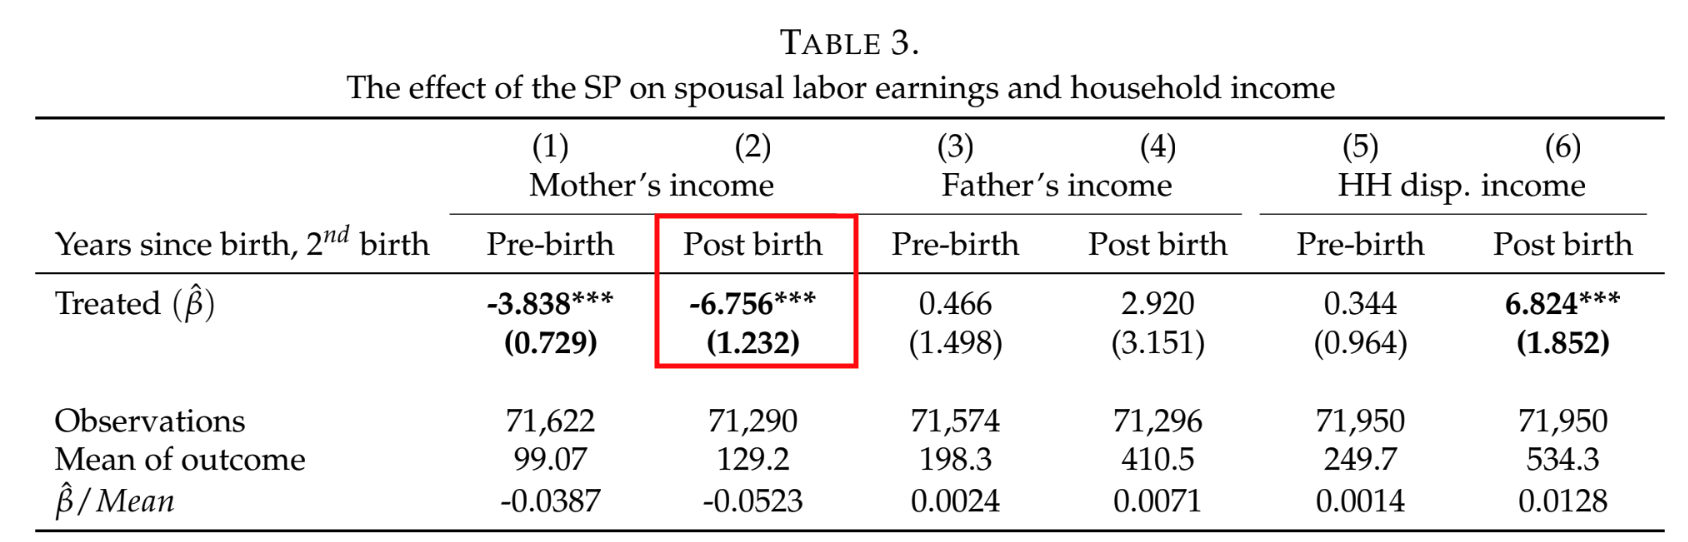
\includegraphics[width=0.9\linewidth]{inputs/fig10-1.png}
\end{figure}
LS declines immediately after- post-birth too - take up of PL 
\end{frame}
% ---------------------------------------------------------------

% ---------------------------------------------------------------
\begin{frame}{Timing of Labor Supply Response}
\begin{figure}
\centering
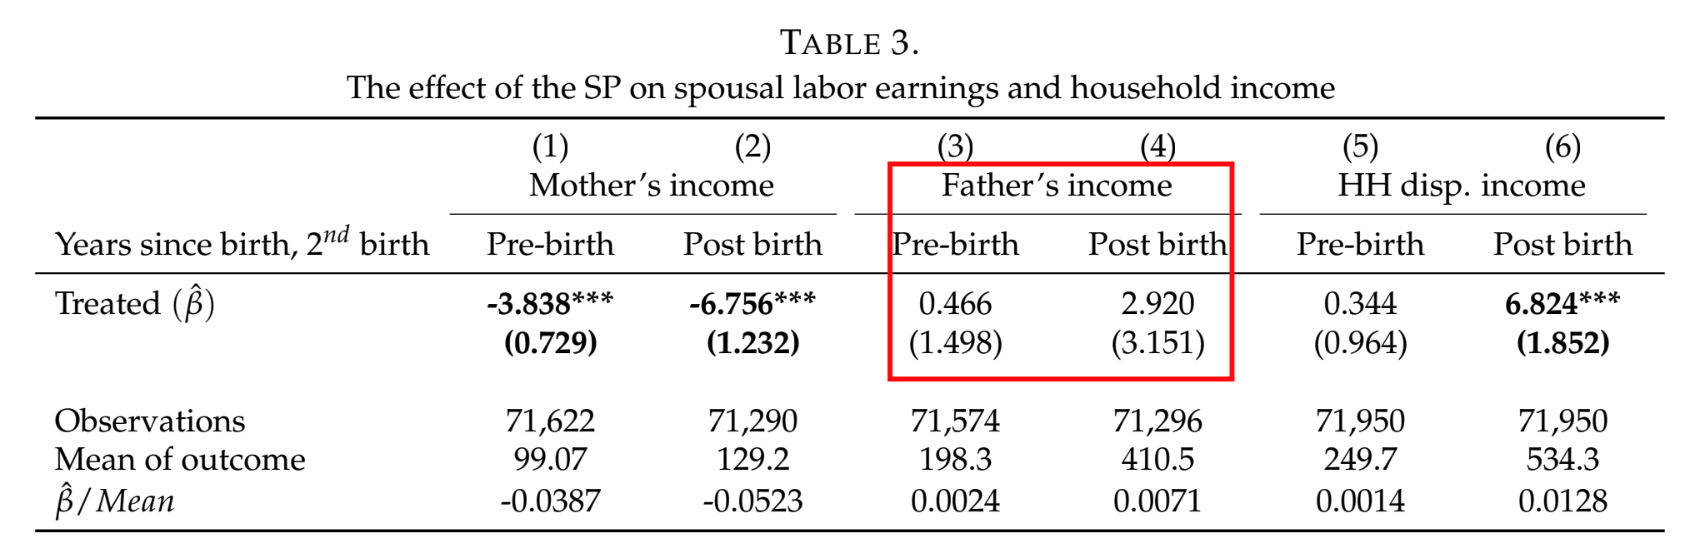
\includegraphics[width=0.9\linewidth]{inputs/fig10-2.png}
\end{figure}
No effect on fathers' LS 
\end{frame}
% ---------------------------------------------------------------

% ---------------------------------------------------------------
\begin{frame}{Timing of Labor Supply Response}
\begin{figure}
\centering
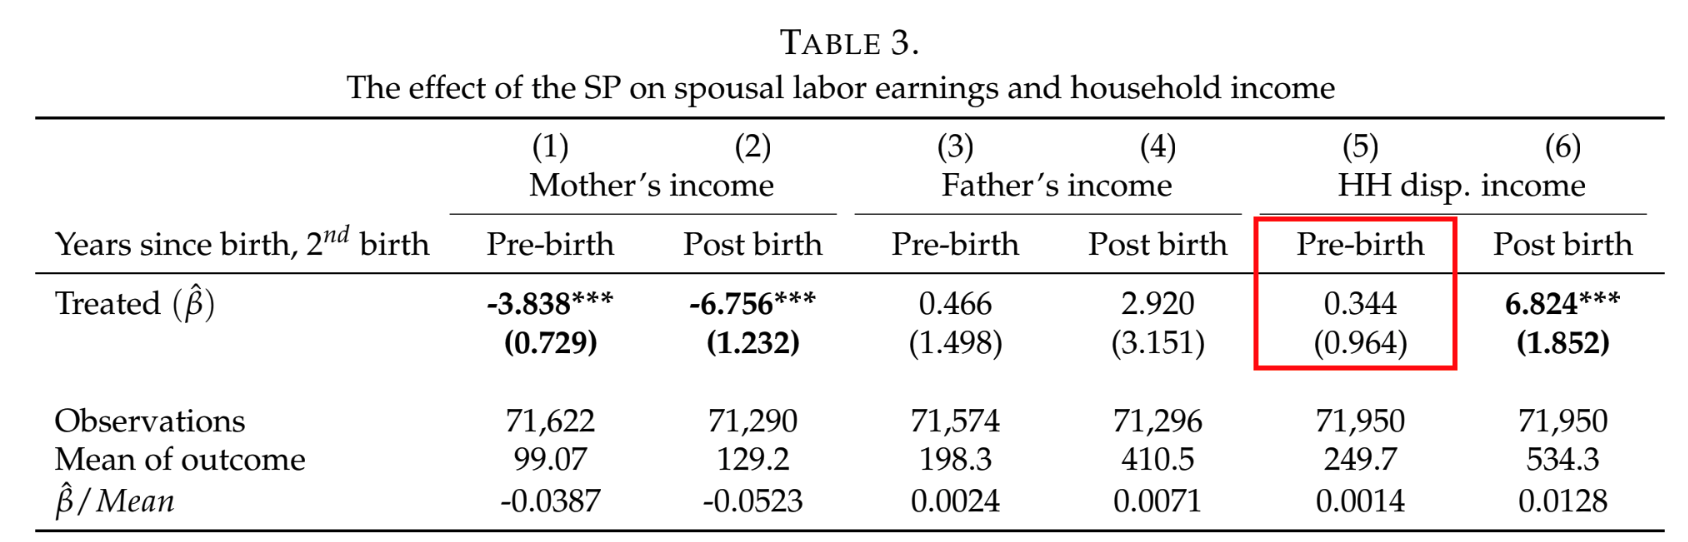
\includegraphics[width=0.9\linewidth]{inputs/fig10-3.png}
\end{figure}
HH disposable income does not decrease pre-birth - paid maternity leave or government transfers
\end{frame}
% ---------------------------------------------------------------

% ---------------------------------------------------------------
\begin{frame}{Timing of Labor Supply Response}
\begin{figure}
\centering
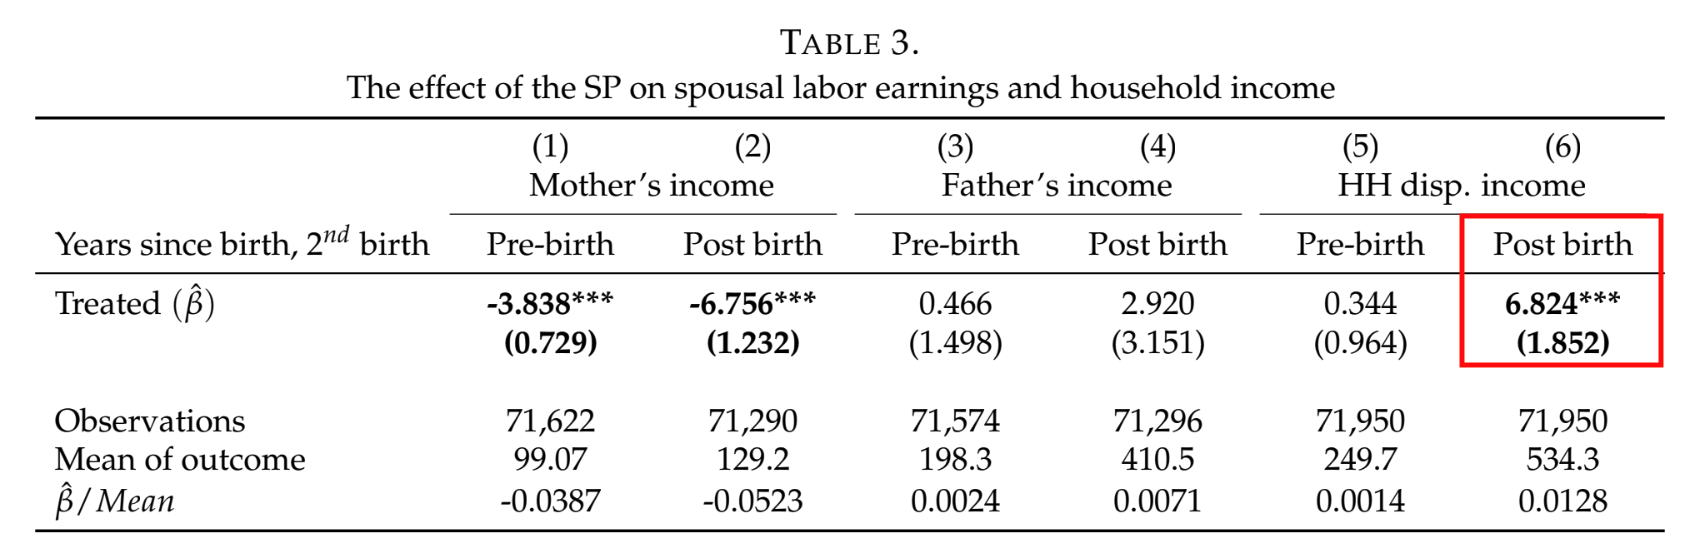
\includegraphics[width=0.9\linewidth]{inputs/fig10-4.png}
\end{figure}
Positive effect of SP HH's post-birth disposable income - mothers on PL
\end{frame}
% ---------------------------------------------------------------

% ---------------------------------------------------------------
\begin{frame}{Timing of Labor Supply Response}
\begin{figure}
\centering
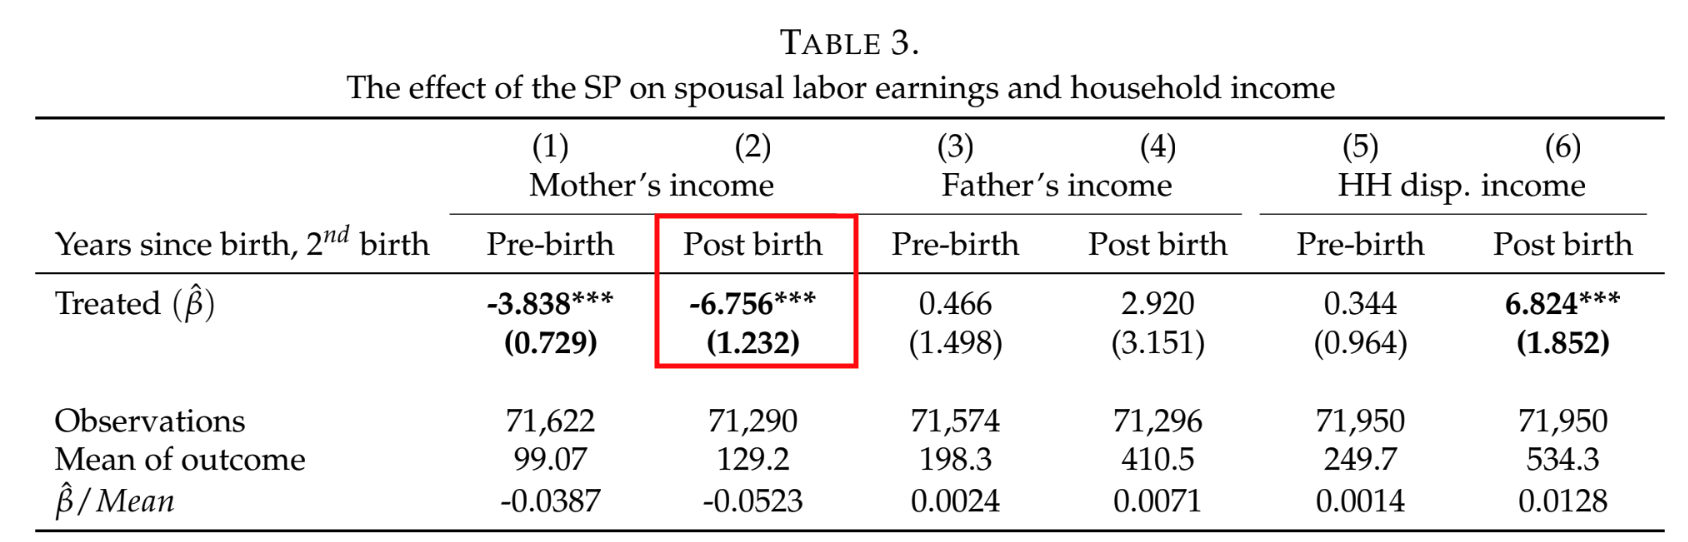
\includegraphics[width=0.6\linewidth]{inputs/fig10-1.png}
\end{figure}
Mothers reduce LS in the year before second birth by nearly 4\% relative to baseline earnings
\end{frame}
% ---------------------------------------------------------------

% ---------------------------------------------------------------
\begin{frame}{Temporal Effect of SP on Maternal Labor Supply}
\begin{figure}
\centering

\includegraphics[width=0.75\linewidth]{inputs/fig11.png}
\end{figure}
Pre-treatement placebo 
\end{frame}
% ---------------------------------------------------------------

% ---------------------------------------------------------------
\begin{frame}{Temporal Effect of SP on Spousal Labor Supply}
\begin{figure}
\centering
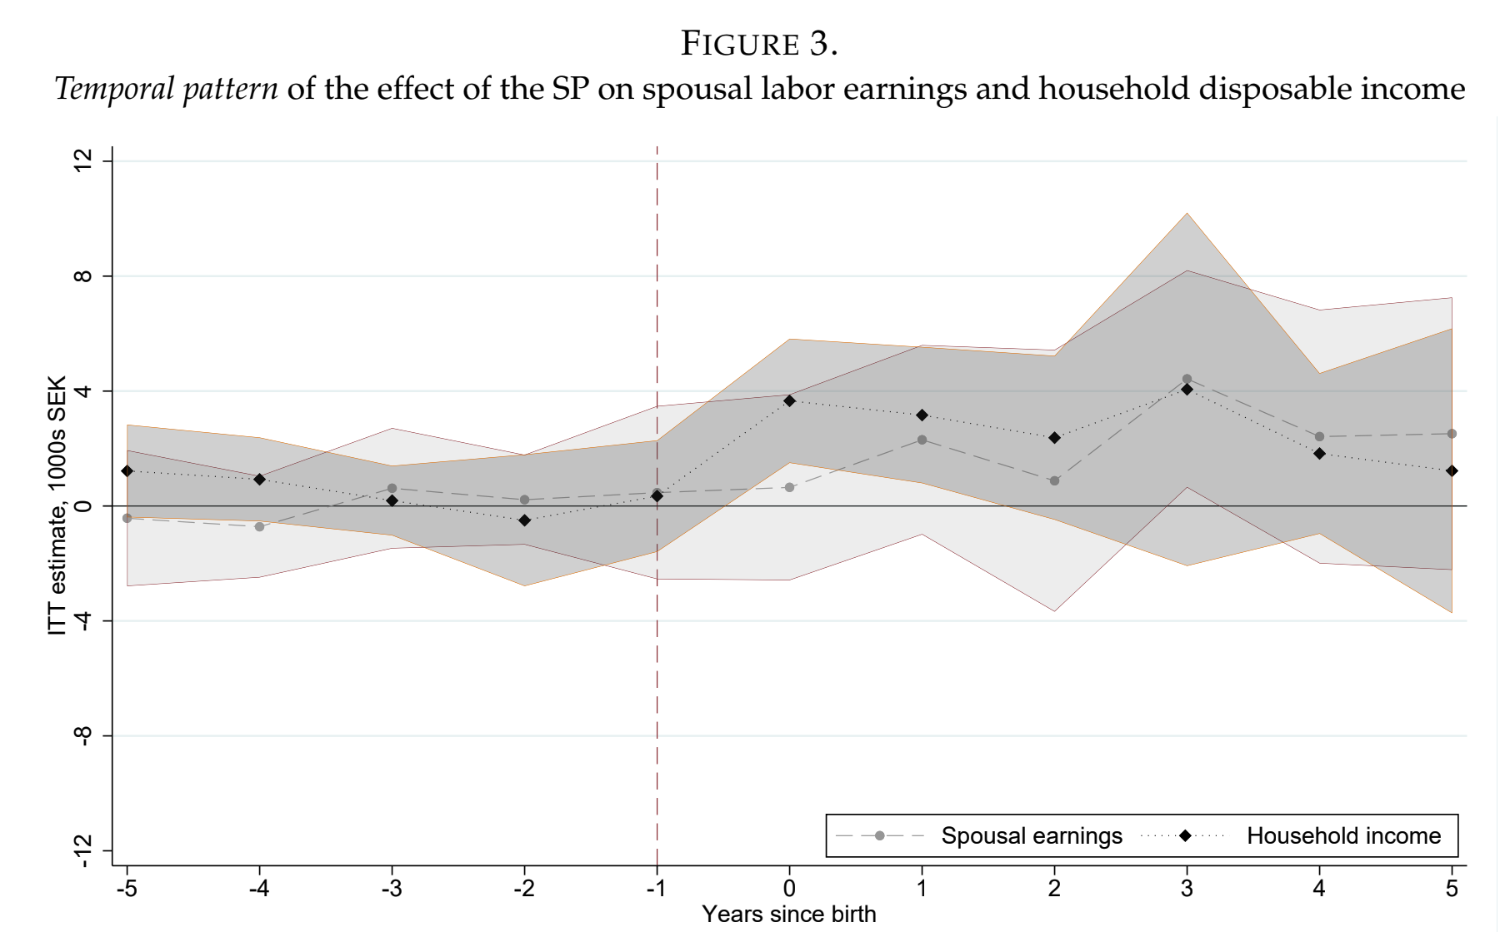
\includegraphics[width=0.75\linewidth]{inputs/fig12.png}
\end{figure}
No effect on fathers' LS - no evidence of substitution
\end{frame}
% ---------------------------------------------------------------


% ---------------------------------------------------------------
\begin{frame}{Heterogeneity by Mother's Earnings}
\begin{figure}
\centering
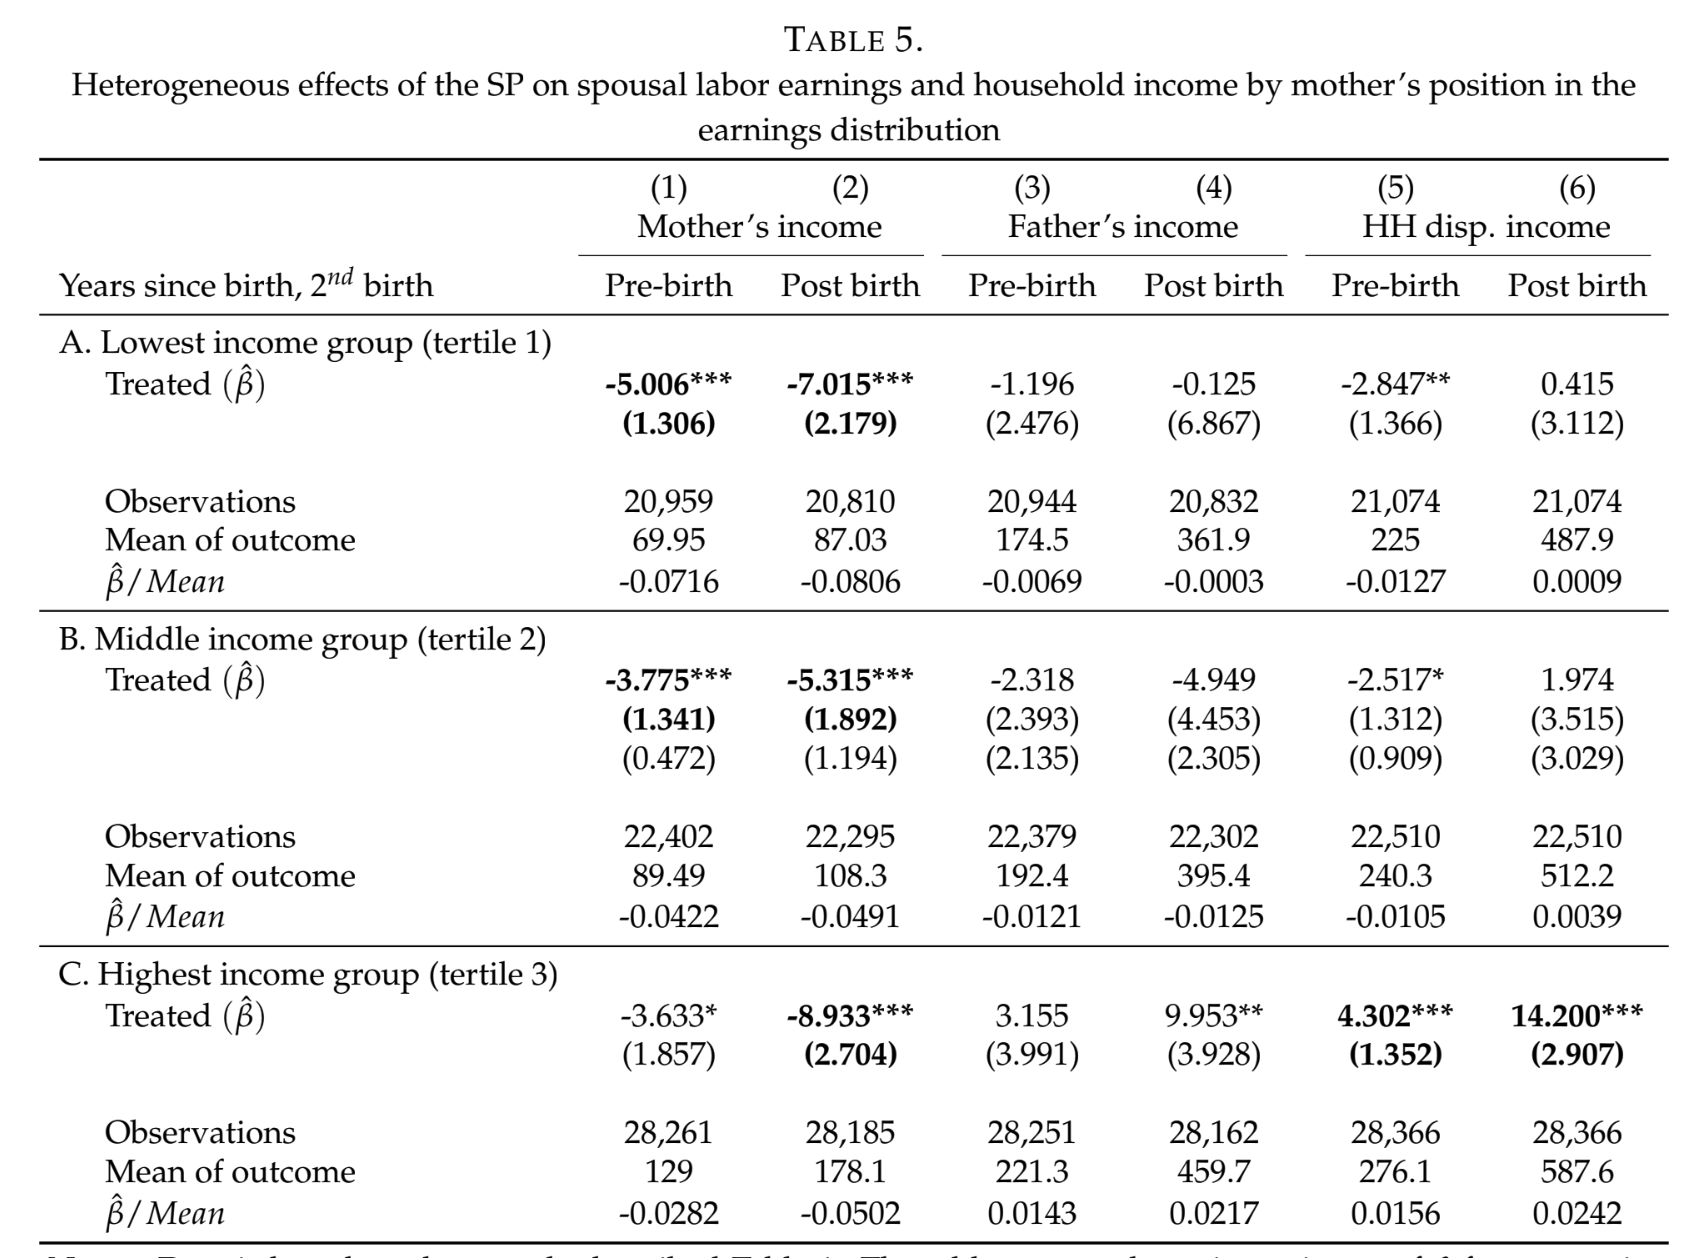
\includegraphics[width=0.6\linewidth]{inputs/fig13.png}
\end{figure}
For high-earning couples, SP increases \emph{specialization}: more maternal home time, more paternal market work in the short run.
\end{frame}
% ---------------------------------------------------------------


% ---------------------------------------------------------------
\begin{frame}{Birth \& Health Outcomes}
\begin{figure}
\centering
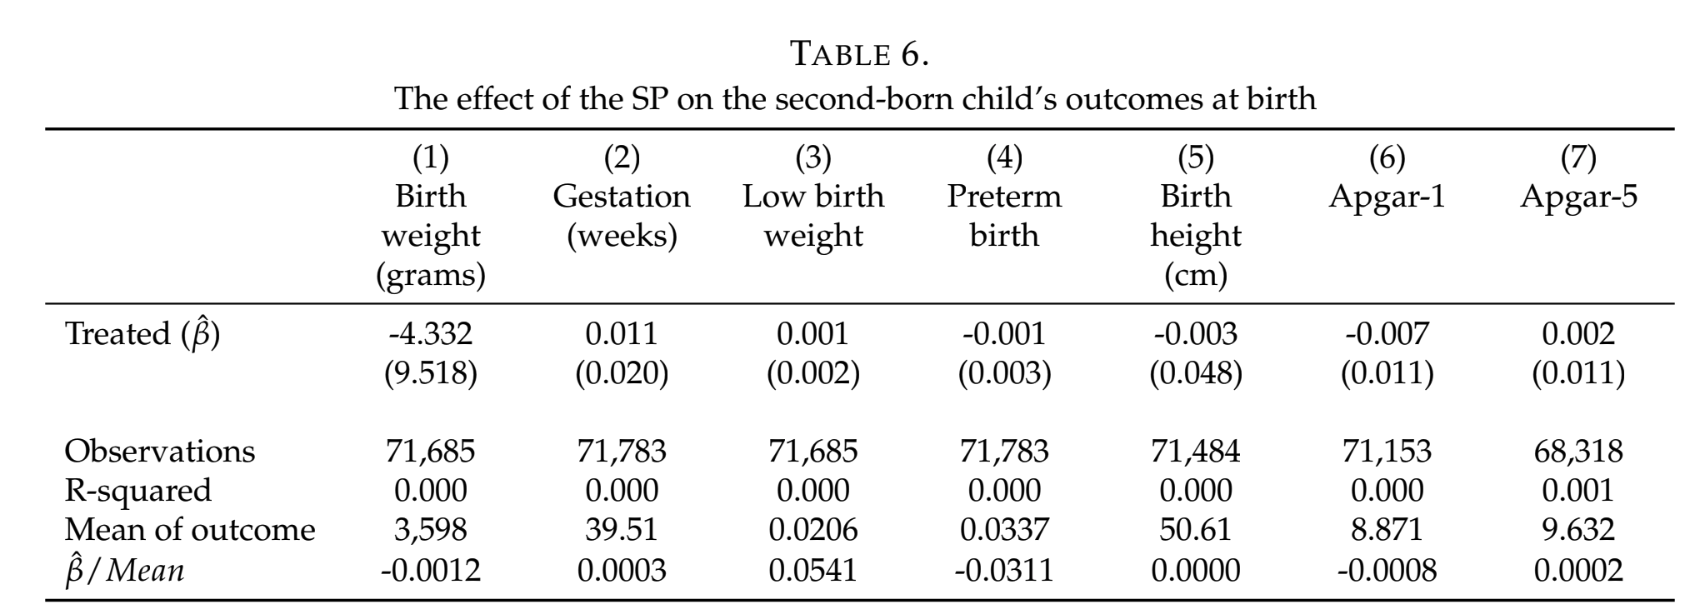
\includegraphics[width=0.9\linewidth]{inputs/fig14.png}
\end{figure}
\end{frame}
% ---------------------------------------------------------------

% ---------------------------------------------------------------
\begin{frame}{Education Outcomes}
\begin{figure}
\centering
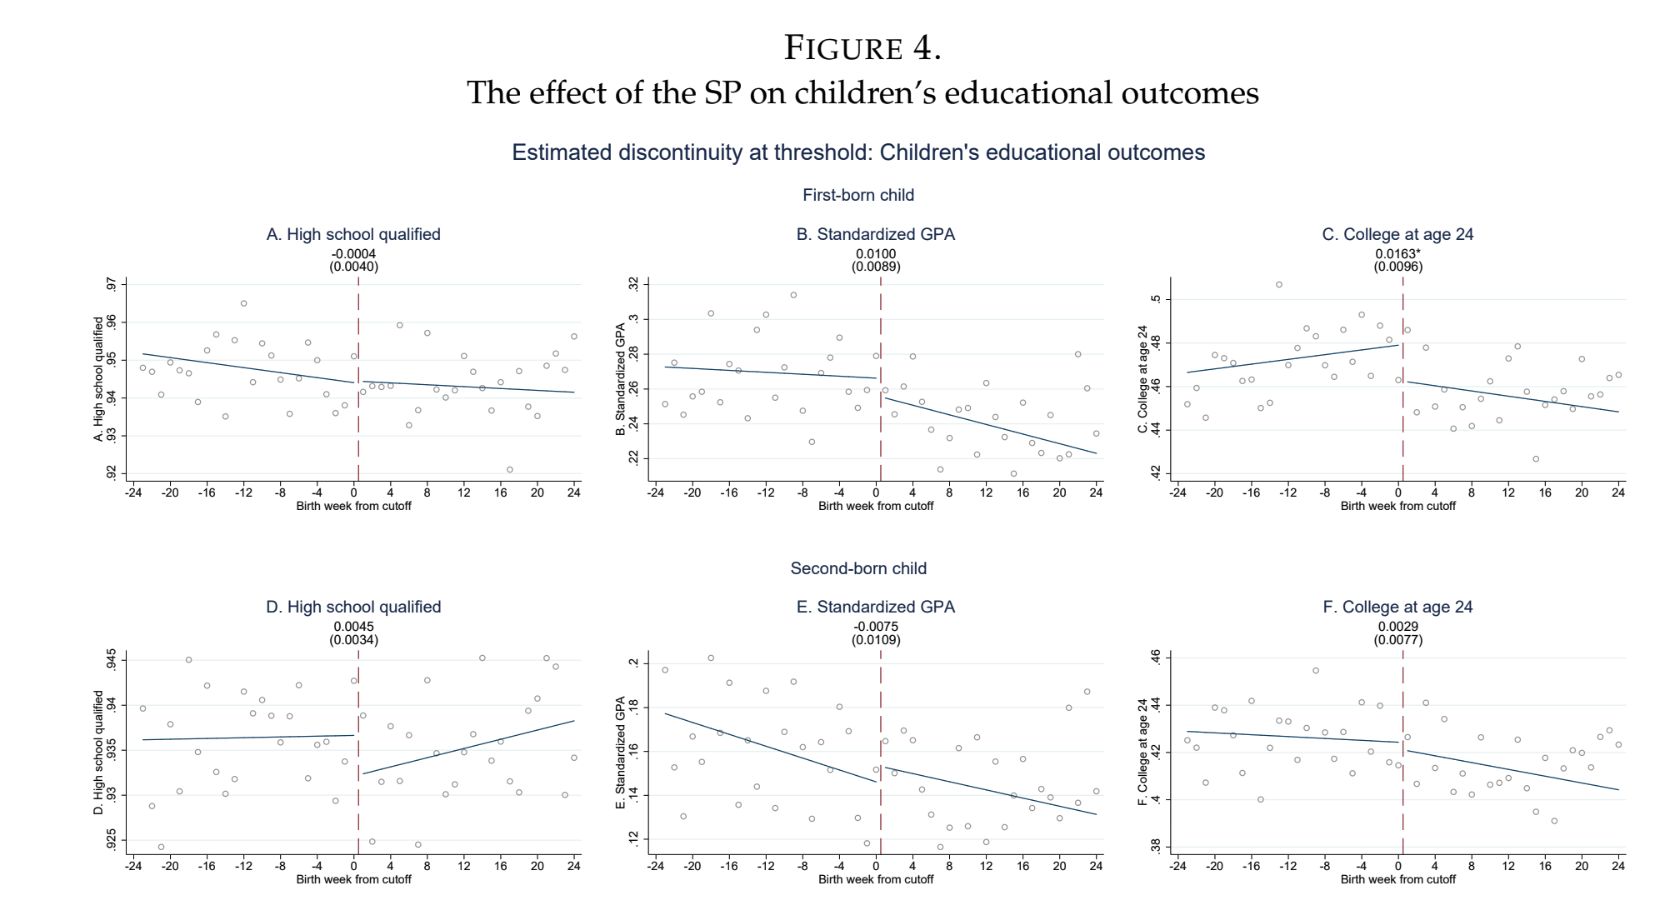
\includegraphics[width=0.95\linewidth]{inputs/fig15.png}
\end{figure}
\end{frame}
% ---------------------------------------------------------------

% ---------------------------------------------------------------
\begin{frame}{Education Outcomes: Older vs Younger Sibling}
\begin{itemize}
    \item First-born children to mothers with SP eligibility are more likely to attain higher
    education
    \item But that there are no impacts for the younger child
    \item Why? \pause Possibly because the older child is younger at the time of the sibling's birth, and thus receives more exclusive maternal time
    \item Time spent with the mother is more important in the early years of life
    \item Later child may not benefit as much from the increased maternal time - compete with the older sibling
    \item Another penalty : Birth order penalty!
\end{itemize}
\end{frame}
% ---------------------------------------------------------------

% ---------------------------------------------------------------
\begin{frame}{Heterogeneity by Mother's Earnings}
\begin{figure}
\centering
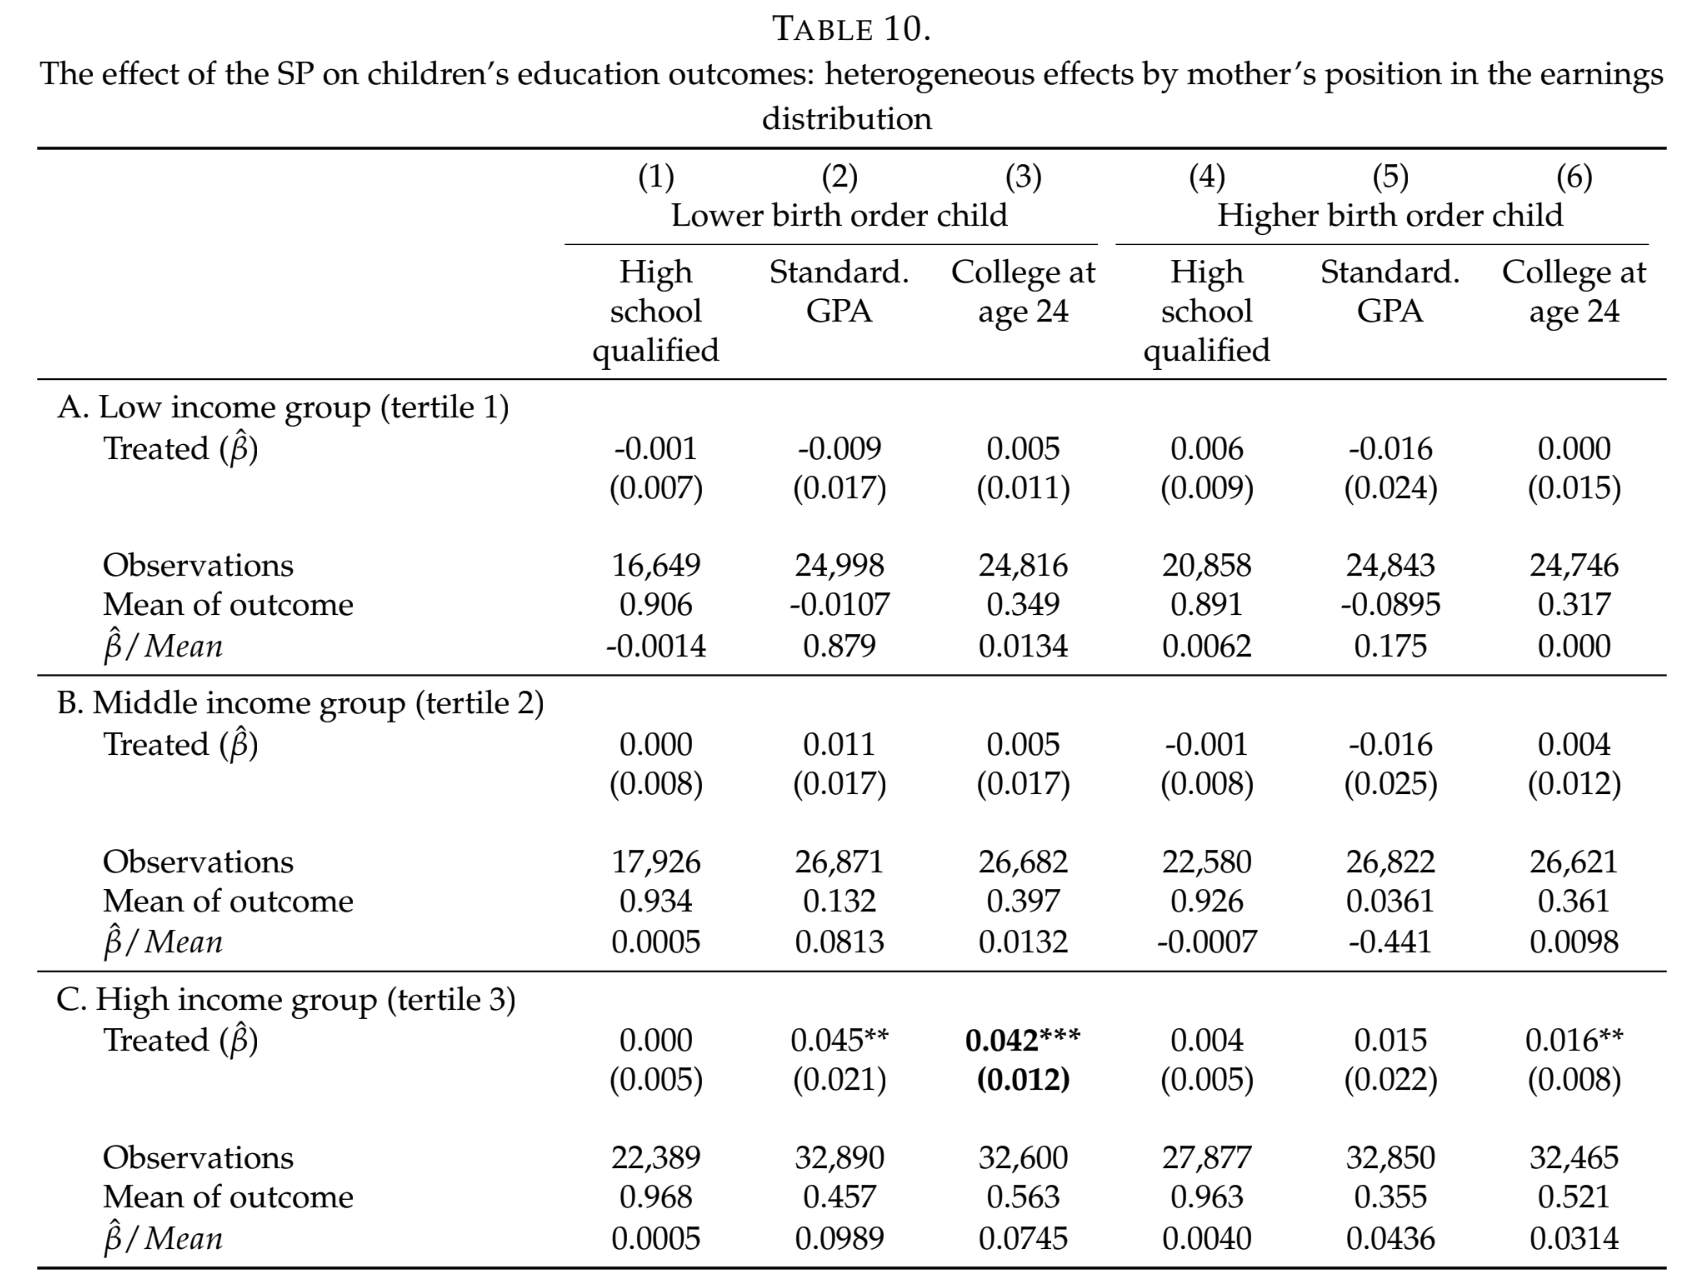
\includegraphics[width=0.7\linewidth]{inputs/fig16.png}
\end{figure}
\small
Recall that maternal LS responses were similar - quality of maternal care? Complementarities of household income and maternal time?
\end{frame}
% ---------------------------------------------------------------


% ---------------------------------------------------------------
\begin{frame}{Heterogeneity by Mother's Earnings}
\begin{figure}
\centering
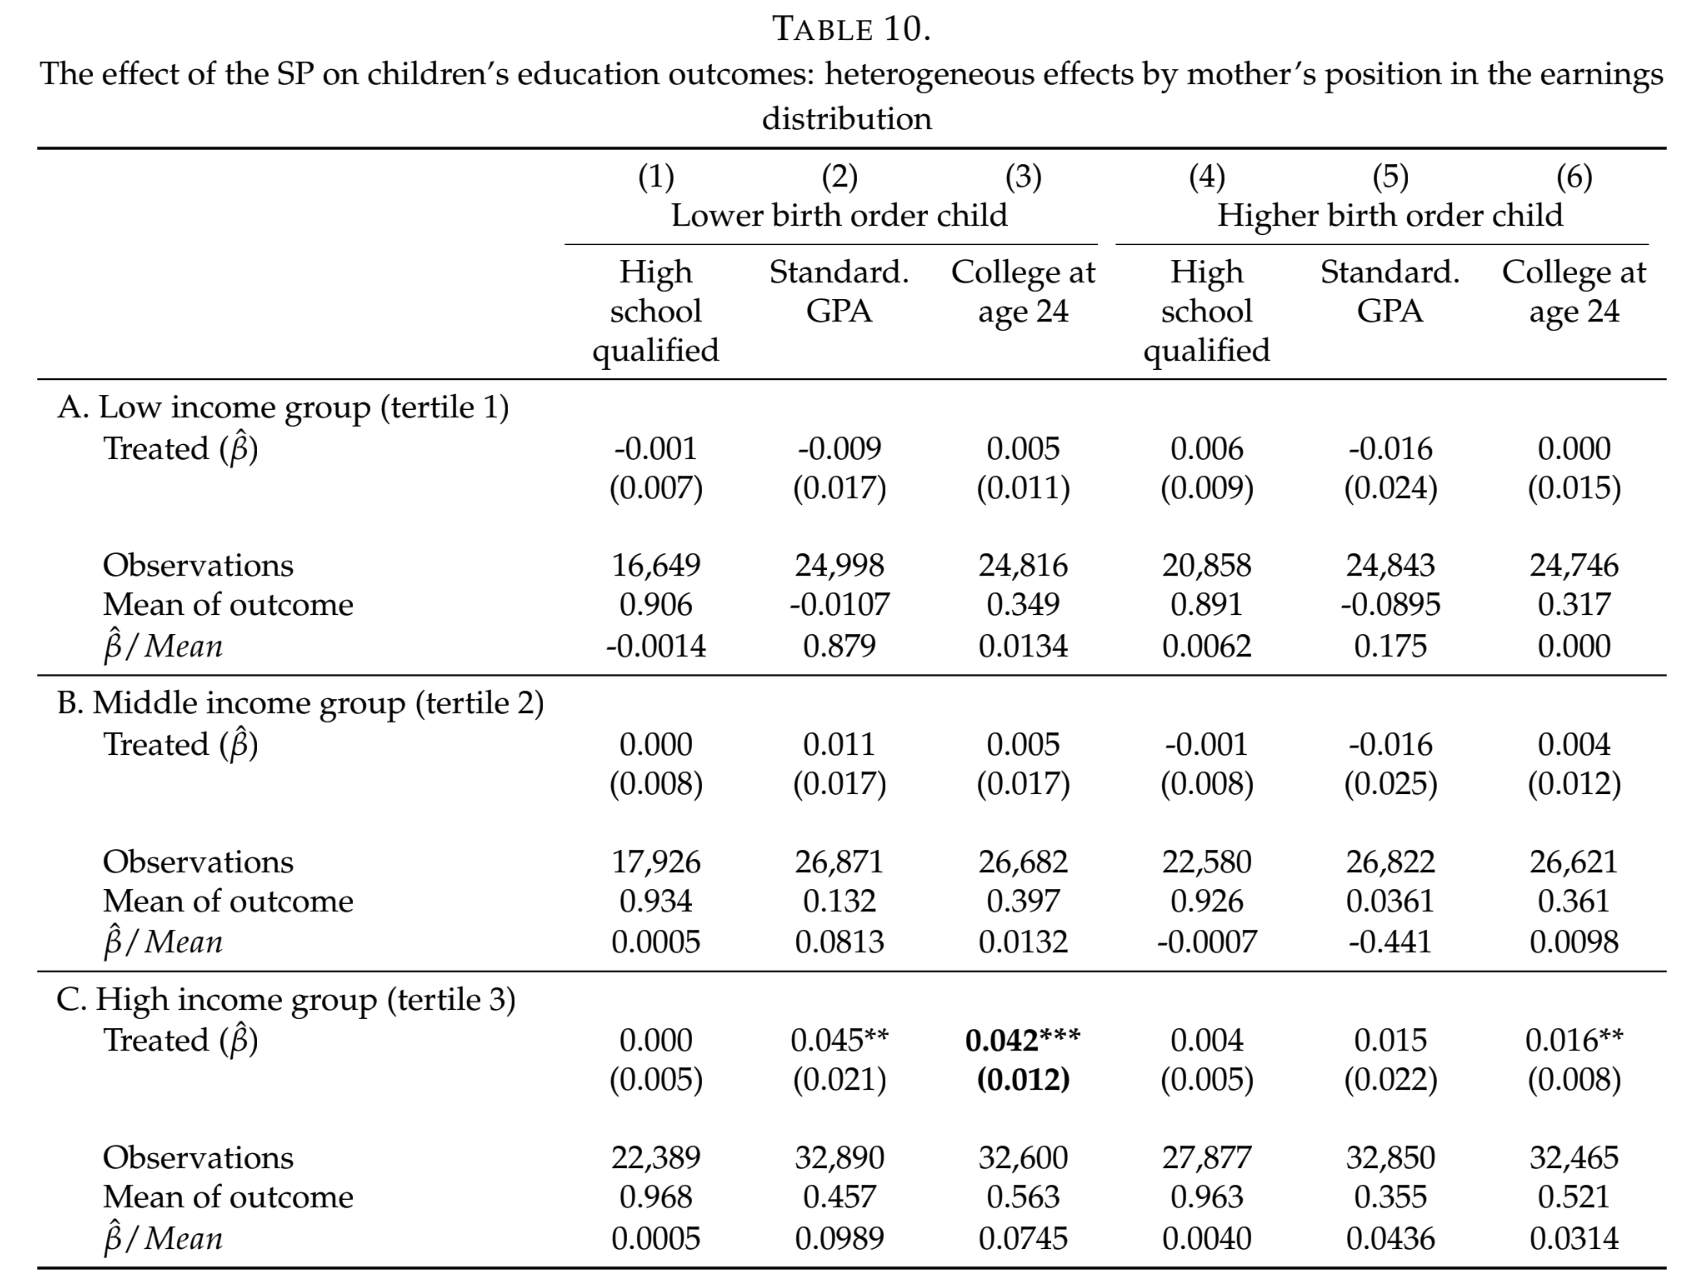
\includegraphics[width=0.55\linewidth]{inputs/fig16.png}
\end{figure}
\small
Recall that maternal LS responses were similar - quality of maternal care? Complementarities of household income and maternal time?
\end{frame}
% ---------------------------------------------------------------

% ---------------------------------------------------------------
\begin{frame}{Conclusions}
\begin{itemize}
  \item SP has clear incentives for mothers to reduce labor supply before and after birth of the subsequent child
  \item No evidence of substitution to fathers' labor supply, except for high-earning couples
  \item SP increases children's schooling performance for the older sibling, especially with high-SES mothers
\end{itemize}
\end{frame}
% ---------------------------------------------------------------



% ---------------------------------------------------------------
\begin{frame}{Interpretation}
\small
\textbf{For parents:} Higher benefit levels (at fixed duration) shift mothers from market to home in the short run; little long-run earnings impact measured; some short-run \emph{specialization} for high-SES couples.\\[0.4em]
\textbf{For children:} The \emph{existing} child gains in schooling (GPA/college), especially with high-SES mothers and at the 24-month threshold—consistent with more \emph{exclusive} maternal time replacing lower-quality care.\\[0.4em]
\textbf{Distributional angle:} The SP can be \emph{regressive} (larger gains among high-SES) and may widen \emph{birth-order gaps}.
\end{frame}
% ---------------------------------------------------------------

\section{When Dad Can Stay Home — AEJ Applied 2024}


% ---------------------------------------------------------------
\begin{frame}{Motivation}
\begin{itemize}
  \item Flexibility at the workplace is increasingly values as an amenity 
    \item Especially for parents with young children facing unpredictable health and care needs (snow days and sick days!) 
    \item And even more so for mothers - on call for domestic household needs 
    \item Goldin (2014) (and others): workplace flexibility could be key to reducing the gender pay gap
\end{itemize}
\end{frame}
% ---------------------------------------------------------------

% ---------------------------------------------------------------
\begin{frame}{What we don't know}
\begin{itemize}
  \item The impact of workplace flexibility on health costs of mothers
    \item Fathers' demand for workplace flexibility and their spillover effects on maternal wellbeing
    \item Role of moral hazard in paid family leave policies and the role of maternal health benefits
\end{itemize}
\end{frame}
% ---------------------------------------------------------------

% ---------------------------------------------------------------
\begin{frame}{This Paper}
\small
\textbf{Persson \& Rossin-Slater (2024).} \emph{When Dad Can Stay Home: Fathers’ Workplace Flexibility and Maternal Health}, \textit{AEJ: Applied Economics}, 16(4):186–219.\\[0.6em]
\begin{itemize}
  \item \textbf{Question:} Does granting \emph{fathers} flexible access to leave improve \textbf{maternal postpartum health}? 
  \item \textbf{Policy:} Sweden’s \textbf{“Double Days”} (Jan 1, 2012) — up to \textbf{30 additional days} of \emph{simultaneous} full-time parental leave in the child’s first year (beyond the baseline 10 days). 
  \item \textbf{Design:} RD–DiD using \emph{share of days eligible} in the first month post-birth around the cutoff
  \item \textbf{Preview:} More paternal flexibility $\Rightarrow$ \textbf{fewer maternal complications} and \textbf{lower anti-anxiety medicine use}
\end{itemize}
\end{frame}
% ---------------------------------------------------------------

% ---------------------------------------------------------------
\begin{frame}{Institutional Background}
\small
\begin{itemize}
    \item 1974: Sweden introduced gender-neutral paid parental leave
  \item Pre-reform: parents could not take paid leave \emph{together} --except \textbf{10 baseline days} in the first 60 days post birth. Why?  
  \item \textbf{2012 reform:} up to \textbf{30 extra} \emph{intermittent} simultaneous leave days in the first year; \emph{no change} to total leave allotment
  \item No advance employer notice required for the second leavetaker if the mother is sick; 
  \item Effectively increases \textbf{temporal flexibility for fathers} on how to allocate the timing of their leave 
\end{itemize}
\end{frame}
% ---------------------------------------------------------------

% ---------------------------------------------------------------
\begin{frame}{Maternal Health Outcomes (Pre-Reform)}
\small
\begin{figure}
\centering

\includegraphics[width=0.6\linewidth]{inputs/fig1.png}
\end{figure}
\end{frame}
% ---------------------------------------------------------------

% ---------------------------------------------------------------
\begin{frame}{Data}
\begin{itemize}
    \item Birth data: all Swedish births 2000-2016 and characteristics, identify singleton births 
    \item Parental leave claims - all leave spells 
    \item Maternal health outcomes - inpatient and outpatient visits, prescriptions filled
\end{itemize}
\end{frame}
% ---------------------------------------------------------------


% \section{Design \& Identification}

% ---------------------------------------------------------------
\begin{frame}{Design Sketch: RD–DD Around Jan 1, 2012}
\small
\begin{itemize}
  \item The goal: isolate variation in \textbf{father's leave flexibility} around Jan 1, 2012 reform to study causal effect on maternal health
  \item Key idea: births just before vs just after Jan 1, 2012 differ in \textbf{eligibility for simultaneous leave} in the first month postpartum
  \item Eg: Dec 31, 2011 birth: only 29 days eligible in first month -- share 29/30 = 0.97 \\
  \item Jan 1, 2012 birth: full 30 days eligible -- share 30/30 = 1.00
  \item Compare outcomes of parents of children born in January - March 2012 and October - December 2011 to those born in same months in 2010, 2009, 2008
\end{itemize}
\end{frame}
% ---------------------------------------------------------------

% ---------------------------------------------------------------
\begin{frame}{Design Sketch: RD–DD Around Jan 1, 2012}
\small
\begin{itemize}
  \item Estimate:
  \[
  Y_{idp} = \alpha_0 + \alpha_1 \textrm{ShareDaysEligible}_{idp} + \alpha_2 1\{d \geq c\} + f(d-c) + 1\{d \geq c\} \times f(d-c) + \theta_p + \varepsilon_{idp}
  \]
\end{itemize}
\end{frame}
% ---------------------------------------------------------------


% ---------------------------------------------------------------
\begin{frame}{Design Sketch: RD–DD Around Jan 1, 2012}
\small
\begin{itemize}
  \item What's different about this design from the usual RDD?
       \begin{itemize}
        \item Running variable is continuous (share of days eligible in month 1)
        \item Treatment is not a binary jump at the cutoff, but a change in the slope of the running variable at the cutoff
    \end{itemize}
    \item Why use the Difference-in-Differences?
        \begin{itemize}
            \item Controls for seasonality in births and health outcomes
        \end{itemize}
    \item What's the identifying assumption?
        \begin{itemize}
            \item No other changes at the date cutoff that differentially affect maternal health outcomes
        \end{itemize}
\end{itemize}
\end{frame}
% ---------------------------------------------------------------

% ---------------------------------------------------------------
\begin{frame}{First Stage: Fathers Use More Leave in Month 1}
\begin{figure}
\centering

\includegraphics[width=0.8\linewidth]{inputs/fig2.png}
\end{figure}
\end{frame}
% ---------------------------------------------------------------


% ---------------------------------------------------------------
\begin{frame}{First Stage: Fathers Use More Leave in Month 1}
\small
\begin{itemize}
  \item Full eligibility $\Rightarrow$ father uses \textbf{any post-baseline leave} \(+\) \textbf{3.9 p.p.} (\textbf{+92\%} at mean). 
  \item Seasonal variation in leave: needed the non-reform years and the DD design
  \item Leave starts to increase at the end of 2011 - consistent with them being eligible 
\end{itemize}
\end{frame}
% ---------------------------------------------------------------

% ---------------------------------------------------------------
\begin{frame}{Maternal Health: Childbirth Complications}
\begin{figure}
\centering
\begin{minipage}{0.45\textheight}

\includegraphics[width=0.45\textheight]{inputs/fig3.png}
\end{minipage}\hfill
\end{figure}
\end{frame}
% ---------------------------------------------------------------


% ---------------------------------------------------------------
\begin{frame}{Maternal Health: Anxiety Medications}
    \begin{figure}
\centering

\includegraphics[width=0.45\textheight]{inputs/fig4.png}
\end{figure}
\end{frame}
% ---------------------------------------------------------------


% ---------------------------------------------------------------
\begin{frame}{Maternal Health: Antibiotic Drugs}
\begin{figure}
\centering

\includegraphics[width=0.45\textheight]{inputs/fig5.png}
\end{figure}
\end{frame}
% ---------------------------------------------------------------

% ---------------------------------------------------------------
\begin{frame}{In Regression Form}
\begin{figure}
    \centering
    
\includegraphics[width=0.5\linewidth]{inputs/fig6.png}
    \end{figure}
    \small
\begin{itemize}
   \item Maternal \textbf{inpatient/outpatient} visit for childbirth complications: \textbf{1.0 p.p.} (\textbf{12\%}).
  \item Mothers with pre-birth medical histories: \textbf{2p.p.} (\textbf{20\%}).
\end{itemize}
\end{frame}
% ---------------------------------------------------------------


% ---------------------------------------------------------------
\begin{frame}{In Regression Form}
\begin{figure}
\centering

\includegraphics[width=0.8\linewidth]{inputs/fig7.png}
\end{figure}
\end{frame}
% ---------------------------------------------------------------

% ---------------------------------------------------------------
\begin{frame}{In Regression Form}
\begin{figure}
\centering

\includegraphics[width=0.5\linewidth]{inputs/fig7.png}
\end{figure}
\begin{itemize}
  \pause \item Maternal anti-anxiety prescription: \textbf{0.2 p.p.} (\textbf{72\%}). 
\item Maternal antibiotic prescription: \textbf{1.5 p.p.} (\textbf{14\%}).
\end{itemize}
\end{frame}
% ---------------------------------------------------------------


% ---------------------------------------------------------------
\begin{frame}{Mechanism: Targeted Co-Presence on Medical Days}
\begin{figure}
\centering

\includegraphics[width=0.8\linewidth]{inputs/fig8.png}
\end{figure}
\end{frame}
% ---------------------------------------------------------------

% ---------------------------------------------------------------
\begin{frame}{Mechanism: Targeted Co-Presence on Medical Days}
\begin{itemize}
 \item Eligibility increases the probability the \textbf{father takes leave on a day} the mother has a medical encounter by \textbf{+0.5 p.p.} (\textbf{+40\%})
  \item \textbf{+1.3 p.p.} (\textbf{+65\%}) if the mother has a pre-birth medical history.
  \item Fathers’ flexibility appears to facilitate \textbf{prompt care} or support on days with domestic health shocks.
\end{itemize}
\end{frame}
% ---------------------------------------------------------------



% \section{Implications \& Discussion}

% ---------------------------------------------------------------
\begin{frame}{Conclusion}
\small
\begin{itemize}
    \item Mother’s environment at home can have significant influence on her well-being
  \item Mothers bear the majority of the cost of a lack of workplace flexibility:
    \begin{itemize}
        \item Both directly - career costs of family formation
        \item But also indirectly - fathers' inflexible leave exacerbates maternal health problems
    \end{itemize}
\item Effects on these maternal health outcomes are
larger in both absolute and relative terms for mothers with a pre-birth medical history
  \item Allow families to decide when it's optimal for both parents to be home - even if that means simultaneous leave
  \item Aside: the United States is the only high-income country with a national PFL policy 
\end{itemize}
\end{frame}
% ---------------------------------------------------------------


% ---------------------------------------------------------------
\begin{frame}{Interpretation}
\begin{itemize}
\item Households face \textbf{stochastic domestic shocks} (e.g., maternal infections, fatigue, stress).
\item Flexibility expands the feasible set: \textbf{occasion-specific} paternal leave generates real health gains even with \emph{modest average days used}.
  \item \textbf{Collective model:} Expanding one spouse’s choice set can raise the other’s welfare via intra-household reoptimization.
  \item Complements child-penalty literature by focusing on \textbf{health spillovers}, not just labor supply.
  \item Baseline rule restricting simultaneous leave to 10 days likely \textbf{forgoes health benefits} to deter moral hazard; need to quantify the trade-off
  \item Policy design matters: Timing, simultaneity, and day-level granularity can be as important as total leave weeks.
\end{itemize}
\end{frame}
% ---------------------------------------------------------------


\end{document}
